% Created 2016-04-23 Sat 00:56
\documentclass[11pt]{article}
\usepackage[utf8]{inputenc}
\usepackage[T1]{fontenc}
\usepackage{fixltx2e}
\usepackage{graphicx}
\usepackage{grffile}
\usepackage{longtable}
\usepackage{wrapfig}
\usepackage{rotating}
\usepackage[normalem]{ulem}
\usepackage{amsmath}
\usepackage{textcomp}
\usepackage{amssymb}
\usepackage{capt-of}
\usepackage{hyperref}
\author{Pan An (A0134556A)}
\date{\today}
\title{CS5214 Assignment 4}
\hypersetup{
 pdfauthor={Pan An (A0134556A)},
 pdftitle={CS5214 Assignment 4},
 pdfkeywords={},
 pdfsubject={},
 pdfcreator={Emacs 24.5.1 (Org mode 8.3.4)}, 
 pdflang={English}}
\begin{document}

\maketitle
\tableofcontents

\section{Matrix Multiplication with GCC}
\label{sec:orgheadline6}

\subsection{Abstract}
\label{sec:orgheadline1}
Large matrix multiplications can be very handy considering 
the limitations of cache and the speed of the the RAM access.
This report is about conducting matrix multiplication with 
low level optimizations. Loop tiling and LLVM optimizations
are used in order to provide an acceptable result for a better
scheduling and work load reduction. I used some methods for 
the analysis of the code efficiency in order not to run the whole thing
over and over. In this document, solution to question 1\textasciitilde{}3 was put in section 1. 
Section 2 is the solution for assembly sse design. Section 3 is the vectorization. 
And section 4 provides the solution for the last question. 

\subsection{Basic Matrix}
\label{sec:orgheadline4}
The first version of matrix multiplication is done with
 two arrays of integers(simply for testing). My computer is 
an Alienware 17 R5, and some of the hardware specifications are listed
in Table. 1:


\begin{center}
\begin{tabular}{lr}
\hline
\hline
Params & Value\\
\hline
Architecture: & x86\(_{\text{64}}\)\\
CPU op-mode(s): & 32-bit, 64-bit\\
CPU(s): & 8\\
Thread(s) per core: & 2\\
NUMA node(s): & 1\\
CPU family: & 6\\
Stepping: & 3\\
CPU MHz: & 901.875\\
BogoMIPS: & 4788.98\\
L1d cache: & 32K\\
L1i cache: & 32K\\
L2 cache: & 256K\\
L3 cache: & 6144K\\
\hline
\end{tabular}
\end{center}
System specification:

\begin{center}
\begin{tabular}{ll}
\hline
Operating System & Ubuntu 14.04\\
RAM & 16GB\\
CPU & Intel\\
\hline
\end{tabular}
\end{center}




Represented below, is my code for basic matrix multiplication:
\begin{verbatim}
for(m=0; m<i; ++m){
    for(n=0; n<k; ++n){
        for(l=0; l<j; ++l){
            result[m*k+n] += mat1[m*j+l]*mat2[l*k+n];
        }
    }
}
\end{verbatim}
The code is not optimized in anyway, and I used array to represent a matrix simply 
because I already forgot how to allocate a 2 dimentional pointer. And this piece of code
is a little bit funny since I messed up the normal order of using m and n. Let's just
ignore that.

For this basic version of matrix multiplication, the settings of the 2 matrixes are:
\(a: 20000\times 30000\),
and \(b: 30000\times 40000\). Where a is mat1 and b is mat2. Later part I will use c to denote the result. 

The verification is done for the multiplication result, and it's under the 
tests folder: \textbf{verify.c}. It's basically just multiplication of matrix then print 
out, nothing more.



\subsubsection{Analysis Methods}
\label{sec:orgheadline2}
In order to push to the limit and be efficient at testing the same time, I used couple methods for the analysis of the whole program:
\begin{enumerate}
\item In order to calculate the running time, I printed the running time  every time \textbf{m} changes.
\item Calculate the average of the printed time, then multiply it with total amount of print that will happen.
\item For loop tiling version of the code(and all the later part), print the running time for every tile.
\end{enumerate}

Here is an example of the printing:

\begin{figure}[htb]
\centering
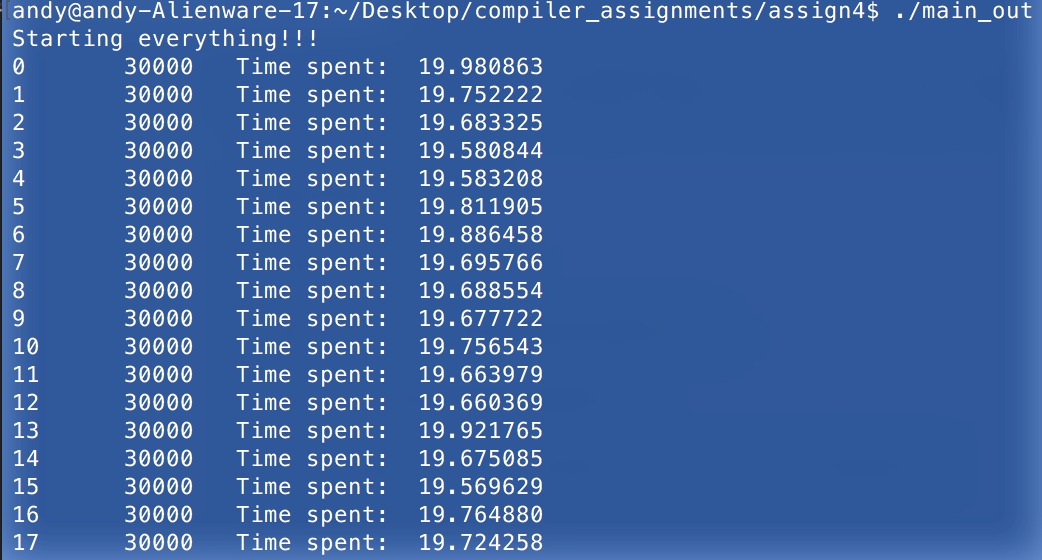
\includegraphics[width=.9\linewidth]{./example.png}
\caption{\label{fig:orgparagraph1}
Example about time monitoring.}
\end{figure}



\subsubsection{Performance}
\label{sec:orgheadline3}
I turned off the graphic desktop to minimize the main system disturbance. 

So the basic matrix multiplication takes about 11GB of RAM. And the whole running process will take approximately 6 days.

\subsection{Loop Tiling}
\label{sec:orgheadline5}
This is pretty much the same idea as the last assignment(God I hope I can get the marks back!!!). You do the loop in a cache friendly way, 
then you save some time. 

Okay here is the code that I used for loop tiling:

\begin{verbatim}
for(m=0;m<i;m+=block_size){
    for(l=0; l<k; l+=block_size){
        #pragma omp parallel for
        for(n=0; n<j; ++n){
            for(mm=0; mm<block_size; ++mm){
                for(nn=0; nn<block_size; ++nn){
                    result[m*k+mm*k+nn+l]+=\
                      mat1[m*j+mm*j+n]*mat2[nn+l+n*k];    
                }
            }
        }
    }
}
\end{verbatim}

I did not use use pragma for vectorization. Later I will explain. With the basic loop tiling, I achieved a better running time of \textbf{1.5} days!!!
Which is a great leap. 

So for loop tiling my original settings for the loop tile is \textbf{100}. I tested with difference lopp sizes, and print time for a single block like this:
\begin{figure}[htb]
\centering
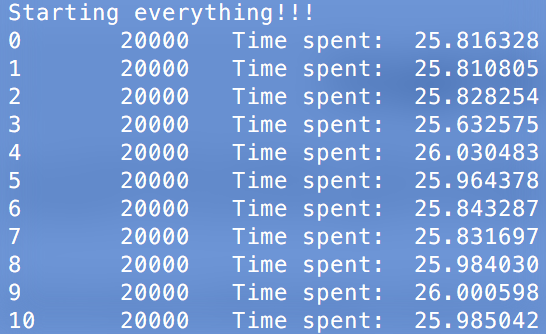
\includegraphics[width=4cm]{./tileexample.png}
\caption{\label{fig:orgparagraph2}
Printing Time.}
\end{figure}

I tested(manually) the running time for different tile sizes. The data of these tiles can be found in the \textbf{.txt} in the assignment folder. As for the limitation of
time I selected the following tile size for testing: \textbf{10, 20, 40, 50, 80, 100, 200, 500, 1000}. 

Performance might vary from tile to tile:

\begin{figure}[htb]
\centering
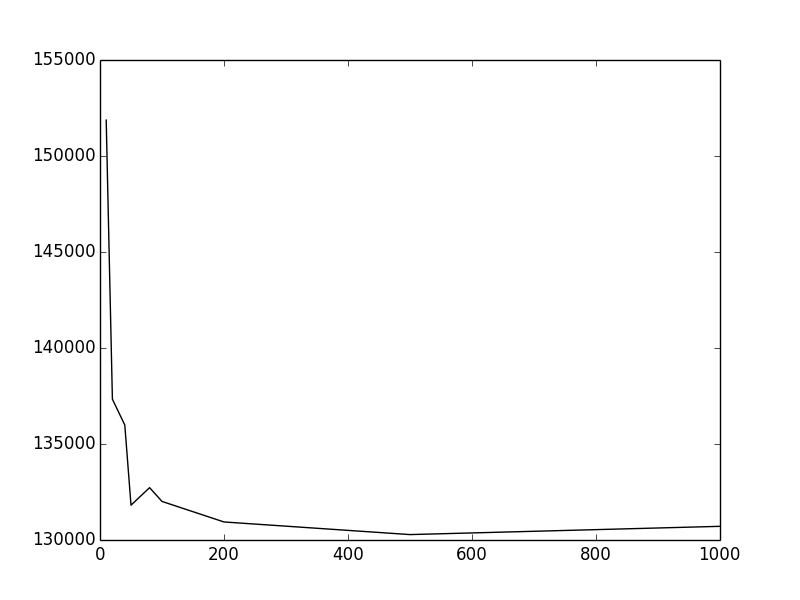
\includegraphics[width=4cm]{./figure.png}
\caption{\label{fig:orgparagraph3}
Printing Time.}
\end{figure}


Funny thing is that you can see that the tile size less than 40 is pretty high. This is because if the tile size is small the performance 
is gonna be like the original one. Noticing here 130000 seconds is around 1.5 days. Which means that no matter what you do, if you want to multiply 
matrixes with 10GB  amount of size, you probably will have to spend so much time with this computer.

\section{Assembly and SSE}
\label{sec:orgheadline7}

Here is a funny story:

Well this part actually took me a lot of time. Because I actually have not really coded in assembly. The only thing that I have coded is in FPGA. And 
my assembly knowledge is all about how computer works and how to optimize C. So I took a course in Coursera and play all the videos in \(\times 2\) speed. 
Then I found out that I just learned X86 assembly. 

Then I read the SSE Instruction set, and wrote some simple code for GCC to compiler, adding one line each time and see what happens with the outcome. 
Again only to find out that the only knowledge I needed was how to use \textbf{\%xmm} registers. So basically going to the class really will help a lot. 

Anyway for this problem, I simplified the target a little. Here is some assumptions that I made:
\begin{itemize}
\item Allocation of the memory is the same to the original problems;
\item Analyzing a full matrix tiling is equal to analyzing the running time of a single tile block;
\item The result of the MM does not affect the analysis of the efficiency;
\item The loading of the result matrix affects the whole program very little;
\item Vectorization can be done by matrix transpose.
\end{itemize}

Since I am using arrays for matrix multiplications, I only have to provide the running test for a single tiling block. Even the matrix is very big, 
matrix transpose actually only takes tens of seconds in memory. Here is how long  a \(30000\times 40000\) matrix is transposed in my computer:
\begin{figure}[htb]
\centering
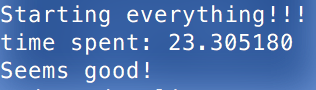
\includegraphics[width=3cm]{./transpose.png}
\caption{\label{fig:orgparagraph4}
Matrix Transpose}
\end{figure}

My assembly code is provided in the \textbf{test/basic.s}. Two functions were written by me are \textbf{main} and \textbf{test\(_{\text{func}}\)}. The program prints
the running time every time a block multiplication is finished. The core process of my code:
\begin{itemize}
\item Load data with MOVPS;
\item Multiplication with MULPS;
\item Add all float numbers in to \%xmm3, with four SHUFPS with 0x39.
\end{itemize}

My estimated time for the whole program is \textbf{1.58} days. Which is not a lot of optimization 
from the first one. 

\section{Vectorization}
\label{sec:orgheadline8}
For vectorization. The original idea is to optimize it with a struts. I compiled with GCC O2, and compared with basic multiplication. I used relatively small 
matrix sizes: \(a: 2000\times 3000\) and \(b: 3000\times 4000\). The original multiplications can finish within 256 seconds. And the optimized version can do in 76\textasciitilde{}77 seconds. 

Compile main/vec.c with \textbf{./vect.sh}. Then run \textbf{./vec.o}



\section{MMIX}
\label{sec:orgheadline11}
Here this question is finally where my reading of The Art of Computer Programming can be put on some use. I copied stuff from TAOCP, so the
machine instruction set will look like this:

\begin{center}
\begin{tabular}{lll}
\hline
\hline
Instruction & Example & Meaning\\
\hline
JL & jl:   \$reg1, \$reg2,location & Jump if reg2(or data) is less than reg1\\
GETA & geta: \$reg,  data & Put the address into register\\
TRAP & trap: \$reg,  data & Write data to the address pointed to by \$reg\\
MUL & mul:  src,  \$dest & Multiply data in src and \$dest, then store in \$dest\\
ADD & add:  src,  \$dest & Add data in src and \$dest, then store in \$dest\\
\# & Comment & Comment after \#.\\
\hline
\end{tabular}
\end{center}


\subsection{Basic Matrix Multiplication}
\label{sec:orgheadline9}

Here I listed some assumptions:
\begin{itemize}
\item There are 9 common registers: rA~rH, and rS;
\item r0 is the register which is always 0;
\item r1 is the register which is always 1;
\item B is the {\bf register} pointing to the bottom of the stack;
\item CP is the register for storing branching information; 
\item Data addressing is the same as x86;
\item From the memory of B, There are three 4 bytes numbers indicating the matrix size x, y, and z, where x and y is the size of the first matrix, 
y and z is the size of the second;
\item Initially rA and rB is the pointer of the two matrix, and rC is the result matrix;
\item System will automatically return when there is no code at all. 
\item The second matrix is already transposed. 
\item No overflow happened. 
\end{itemize}

The following is the assembly code:
\begin{verbatim}
MAIN:
    MUL   $r0, $rD           # m,n,k
    MUL   $r0, $rE
    MUL   $r0, $rF
MULTIPLY:
    MUL   $rS, $r0
    GETA  $rG, ($rA,$rD,4)   # this is comment, loading 
    GETA  $rH, ($rB,$rF,4)
    MUL   $rG, $rH
    ADD   $rH, $rS
    ADD   $r1, $rD
    JL    -4($B), $rD, MULTIPLY
    GETA  $rF,  $rH
    MUL   ($B), $rH
    TRAP  $rS, ($rC,$rH,4)
    ADD   $r1, $rF
    MUL   $r0, $rD
    JL    -4($B), $rE, MULTIPLY
    GETA  $rE,  $rH
    MUL   -8($B), $rH
    JL    -8($B), $rF, MULTIPLY
\end{verbatim}

There might be bugs in the above code since I did not use any simulator. 


\subsection{Pipelining}
\label{sec:orgheadline10}

Here is the software pipelining example for the machine.

\begin{verbatim}
for n, 0, x-1:
    for m, 0, z-1:
        temp = a[n,:]*b[:,m]
        c[n, m] = sum(temp)
\end{verbatim}

In the above code, temp is a list of numbers of each 2 multiplies to each other coming from a and b. 
The sum is to do the summation from all the data in temp. 
The pipeline runs independent multiplication first to make sure that stalling does not affect the whole procedure. 
\end{document}
